\documentclass[11pt,letterpaper]{article}
\usepackage{amsmath,helvet,fancyhdr,bm}
\usepackage[hidelinks]{hyperref}
%\usepackage{cite,url,color}
\usepackage{url,color}
\usepackage{lipsum}
\usepackage{graphicx}
\usepackage{geometry}
\usepackage{floatrow}
\usepackage{multirow}
\floatsetup[table]{capposition=top}
\usepackage{wrapfig}
\usepackage[square,numbers,sort&compress]{natbib}
\usepackage{subfigure}
\usepackage{booktabs}



\usepackage{tikz}
\DeclareRobustCommand*\state[1]{\tikz[baseline=(char.base)]{\node[shape=circle,draw,inner sep=1.2pt] (char) {\tiny{#1}};}}



%\geometry{verbose,a4paper,tmargin=3.4cm,bmargin=3.0cm,lmargin=2.8cm,rmargin=2.3cm,headheight=3cm,headsep=0.1cm,footskip=1cm}
\geometry{nomarginpar,verbose,a4paper,tmargin=2cm,bmargin=2.0cm,lmargin=2cm,rmargin=2cm,headheight=1cm,headsep=0.8cm,footskip=1.2cm}


\renewcommand{\refname}{\large\textbf{References}}
\pagestyle{fancy}
%\renewcommand{\headrulewidth}{0.6pt}

\fancyfoot{} % clear all footer fields
\fancyhead{} % clear all header fields

\fancyhead[LO]{\small\textbf{Name of first author (Example: Last, F. M.)}}
\fancyhead[RO]{\small\textbf{Short title here}}
\fancyfoot[RO]{\small \textbf{\thepage}}
\fancyfoot[LO]{\small{\textbf{IWDP 2024}}}

%\fancyfoot[LO]{\small{$\bm{13^{\text{th}}}$\textbf{ IWDP -- June 10-13, 2024 -- Ann Arbor, Michigan (USA)}}}

\fancypagestyle{plain}{%
\fancyhf{} % clear all header and footer fields

\fancyhead[C]{\small\textbf{June 10-14, 2024}}
\fancyhead[R]{\small\textbf{Ann Arbor, Michigan}}
%\fancyhead[L]{\small{$\bm{13^{\text{th}}}$\textbf{International Workshop \\ on Detonation for Propulsion}}}
\fancyhead[L]{\small{\textbf{IWDP 2024}}}
\fancyfoot[R]{\small \textbf{\thepage}}
\fancyfoot[L]{\small\textbf{Correspondence to: author@institution.edu}}
}






%%%%%%%%%%%%%%%%%%%%%%%%%%%%%%%%%%%%%% FORMAT SECTIONS
\usepackage{titlesec}
\usepackage{xcolor}
\definecolor{seccol}{rgb}{0.05, 0.15, 0.7} % this defines the color of section titles

\titlespacing*{\section}{0pt}{1ex}{0.5ex}
\titlespacing*{\subsection}{0pt}{1ex}{0.5ex}
\titlespacing*{\subsubsection}{0pt}{0.3ex}{0.3ex}


\titleformat{\section}{\color{seccol}\normalfont\normalsize\bfseries}{\color{seccol}\arabic{section}}{1ex}{}

%\titleformat{\subsection}{\color{seccol}\normalfont\normalsize\bfseries}{\color{seccol}\arabic{section}.\arabic{subsection}}{1ex}{}
\titleformat{\subsection}{\color{seccol}\normalfont\normalsize\itshape\centering}{\color{seccol}\arabic{section}.\arabic{subsection}}{1ex}{}

%\titleformat{\subsubsection}{\color{seccol}\normalfont\normalsize\bfseries}{\color{seccol}\arabic{section}.\arabic{subsection}-\Alph{subsubsection}}{1ex}{}

\setlength\parindent{0ex}

%%%%% reformat title
\makeatletter
\def\@maketitle{%
  \newpage
  \null
  %\vskip -4em%
  \begin{center}%
  \vskip -2em%
  \let \footnote \thanks
    {\LARGE \bf \@title \par}%
    \vskip 1.5em%
    {\large
      \lineskip .5em%
      \begin{tabular}[t]{c}%
        \@author
      \end{tabular}\par}%
    \vskip 1em%
    %{\large \@date}%
    \date{}
  \end{center}%
  \par
  \vskip 1em
  }
\makeatother





\usepackage{caption}
\captionsetup[figure]{labelfont={bf},name={Fig.},labelsep=period,font={footnotesize,bf}}
\captionsetup[table]{labelfont={bf},name={Table},labelsep=period,font={footnotesize,bf}}
\setlength{\abovecaptionskip}{3pt}
\setlength{\belowcaptionskip}{0pt}
%\setlength{\intextsep}{100pt}
\setlength{\textfloatsep}{3pt}


\renewcommand{\bibfont}{\small}
\let\oldbibliography\thebibliography
\renewcommand{\thebibliography}[1]{
  \oldbibliography{#1}
  \setlength{\itemsep}{0.2\itemsep}
  \setlength{\baselineskip}{\baselineskip}
  \setlength{\lineskiplimit}{-\maxdimen}
}


%%%%%%%%%%%%%%%%%%%%%%%%%%%%%%%%%%%%%%%%%%%%%%%%%%%%%%%%%%
%%%%%%%%%%%%%% Title and author information %%%%%%%%%%%%%%
%%%%%%%%%%%%%%%%%%%%%%%%%%%%%%%%%%%%%%%%%%%%%%%%%%%%%%%%%%
\title{Title of Work, with Initial Capitals}

% \author{Author Name\\
% Organization\\
% City, State/Province, Country}

\usepackage{authblk}
\author[1]{First Last of Author A}
\author[2]{First Last of Author B}
\author[1]{First Last of Author C}
\affil[1]{Department of Frozen Land, University of South Pole}
\affil[2]{Department of Icicle Engineering, University of North Pole}



%%%%%%%%%%%%%%%%%%%%%%%%%%%%%%%%%%%%%%%%%%%%% Document begins
\begin{document}


\maketitle


\section{Author Instructions for 13th IWDP Abstracts}
The abstract must be submitted by using this \textbf{Latex template} or the corresponding \textbf{MS Word template} that can be found the meeting website. Submission should be between 300 and 500 words in length. Final submission should be converted and uploaded as a PDF File. LaTeX source files or the original MS Word file will not be accepted.  The abstract should be submitted following the file name convention: \emph{last\_first.pdf}. Templates margins and text area are set so printed abstracts fit best to the A4 ISO paper size and should not be changed. Font size and type should not be changed. Please also do not change the position of the first line of the title. Abstract submission information can be found on the meeting webpage at \textbf{aero.engin.umich.edu/iwdp2024}. Abstract should be submitted for consideration of either the oral presentation or poster; please indicate your selection in the abstract submission form.

 

Note that headers and footers for the title page are different from those of pages 2 onward. Headers of the title page and footers of other pages must not be changed.
Only the left footer of the title page and the headers of other pages must be changed according to the following rules:
\begin{itemize}
    \item For the title page: left foot: indicate the correspondence details; center foot: leave empty; right foot: leave unchanged
    \item  For other pages: left header: indicate the first author name (see example); center header: leave empty; right header: indicate the short title of your extended abstract.
\end{itemize}
LaTex typesetting is strongly encouraged.

To cite the work used in the paper, please use \cite{Bykovskii2006, kailasanath2000review, Lu2014review}


\section{Author Instructions for 13th IWDP Short Paper}

The short paper must be submitted by using this \textbf{Latex template} or the corresponding MS Word template. Submission should be no more than 5 pages in total length, including figures, tables and citations. An opening abstract is not required for the short paper. Final submission should be converted and uploaded as a PDF File. LaTeX source files or the original MS Word file will not be accepted.  The abstract should be submitted following the file name convention: ``\emph{last\_first.pdf}''. Templates margins and text area are set so printed abstracts fit best to the to the A4 ISO paper size and should not be changed. Font size and type should not be changed. Please also do not change the position of the first line of the title. Final short paper submission information can be found on the meeting webpage at \textbf{aero.engin.umich.edu/iwdp2024}. Final short paper submission is required only for oral presentations. 


Do not enter any copyright statement on the abstract: a general copyright statement will be added by the editors in the IWDP electronic proceedings.


%
Note that headers and footers for the title page are different from those of pages 2 onward. Headers of the title page and footers of other pages must not be changed.
Only the left footer of the title page and the headers of other pages must be changed according to the following rules:
\begin{itemize}
    \item For the title page: left foot: indicate the correspondence details; center foot: leave empty; right foot: leave unchanged
    \item  For other pages: left header: indicate the first author name (see example); center header: leave empty; right header: indicate the short title of your extended abstract.
\end{itemize}
LaTex typesetting is strongly encouraged.

To cite the work used in the paper, please use \cite{Bykovskii2006, kailasanath2000review, Lu2014review}


%%%%%%%%%%%%%%%%%%%%%%%%%%%%%%%%%%%%%%%
\section{Some examples of equations, figures and tables}
%%%%%%%%%%%%%%%%%%%%%%%%%%%%%%%%%%%%%%%

%%%%%%%%%%%%%%%%%%%%%%%%%%%%%%%%%%%%%%%
\subsection{An example of an equation}

The differential form of conservation equations of mass can be written as:
%
\begin{align}
\frac{\mathrm{D}\rho}{\mathrm{D}t} + \rho \nabla \cdot \mathbf{u} = 0
\end{align}

%%%%%%%%%%%%%%%%%%%%%%%%%%%%%%%%%%%%%%%
\subsection{Examples of Figures}

Figure~\ref{fig:figure1} and Fig.~\ref{fig:figure2} are example of a full width and a test wrapped figure, respectively. 


\begin{figure}[t]
\centering
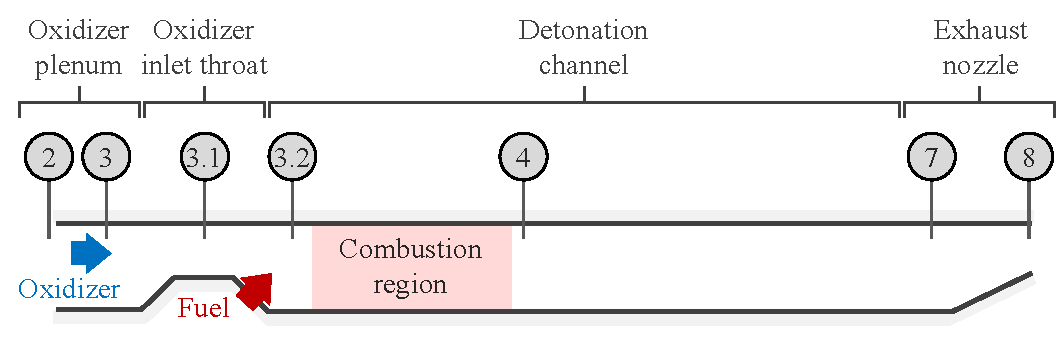
\includegraphics[width=0.65\columnwidth,trim = 0 0 -2 0,clip]{figures/figure1.pdf}
\caption{Example of a full width figure.}
\label{fig:figure1}
\end{figure}



\lipsum[1-2]

\begin{wrapfigure}{r}{0.25\textwidth}
\centering
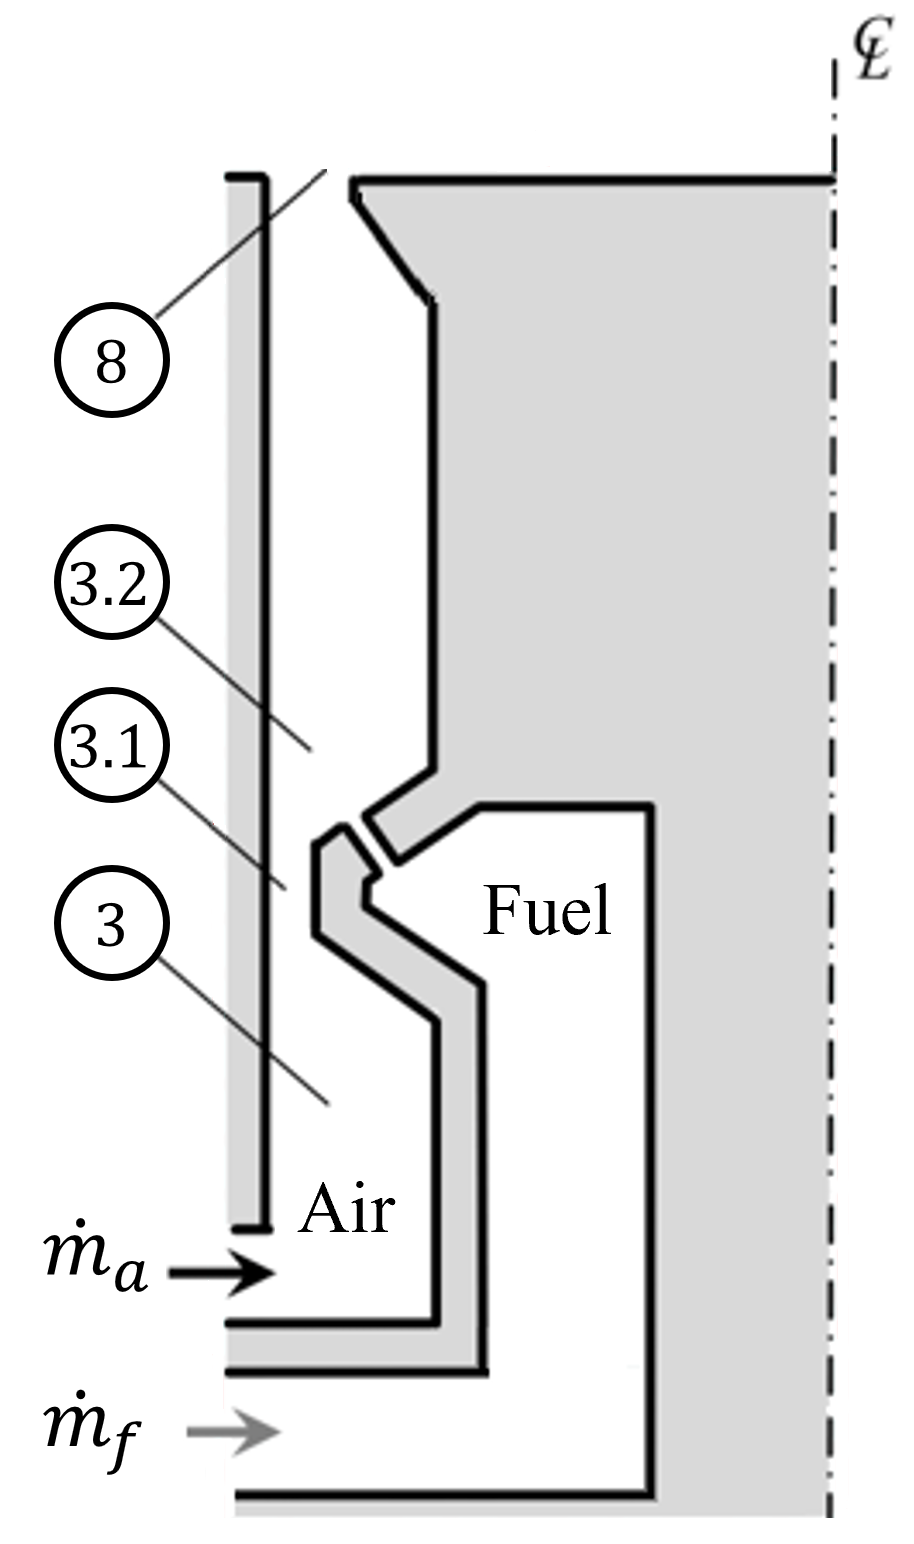
\includegraphics[width=\linewidth]{figures/figure2.png} 
\caption{Example of figure with wrapped text.}
\label{fig:figure2}
\end{wrapfigure}

\lipsum[3-5]

%%%%%%%%%%%%%%%%%%%%%%%%%%%%%%%%%%%%%%%
\subsection{Examples of Tables}

An example of a table is given in table~\ref{tab:states}.


\begin{table}[t]
\begin{center}
\small
\begin{tabular}{ ccc } 
 \toprule 
 {\bf State/Location} & {\bf Ramjet/Scramjet} & {\bf Turbojet/Turbofan}  \\ 
 \hline 
 \state{0} & Ambient & Ambient/Diffuser Inlet \\ 
 \state{1} & End of External Compression  & Compressor Inlet  \\ 
 \state{2} & End of Inernal Compression & Compressor Outlet \\ 
 \state{3} & Combustor Plenum/Isolator & Combustor Plenum \\ 
 \state{3.1} & Oxidizer Inlet Throat & Oxidizer Inlet Minimum Area \\ 
 \state{3.2} & Combustor Channel & Combustor Channel \\ 
 \state{4} & Combustor Outlet & Combustor Outlet \\ 
 \state{5} & -- & Turbine Outlet \\ 
 \state{6} & -- & Afterburner Inlet \\ 
 \state{7} & Start of Nozzle & Afterburner Outlet/Start of Nozzle \\ 
 \state{8} & Nozzle Throat & Nozzle Throat  \\ 
 \state{9} & Nozzle Outlet & Nozzle Outlet \\ 
 \state{10} & Expanded air & --  \\ 
 \bottomrule
\end{tabular}
\caption{\label{tab:states} Description of state location notation in air-breathing engines.}
\end{center}
\end{table}
%


%%%%%%%%%%%%%%%%%%%%%%%%%%%%%%%%%%%%%%%%
\section{Conclusions}
%%%%%%%%%%%%%%%%%%%%%%%%%%%%%%%%%%%%%%%%
Please add a conclusion to summarize the main outcomes of this work.

%\lipsum[1-4]

\bibliographystyle{plain}
\bibliography{library.bib}


\end{document}
